\documentclass[svgnames]{article}     % use "amsart" instead of "article" for AMSLaTeX format
%\geometry{landscape}                 % Activate for rotated page geometry

%\usepackage[parfill]{parskip}        % Activate to begin paragraphs with an empty line rather than an indent

\usepackage{graphicx}                 % Use pdf, png, jpg, or eps§ with pdflatex; use eps in DVI mode

%maths                                % TeX will automatically convert eps --> pdf in pdflatex
\usepackage{amssymb}
\usepackage{amsmath}
\usepackage{esint}
\usepackage{geometry}
\setcounter{secnumdepth}{5}
\setcounter{tocdepth}{5}

\usepackage{pgfplots,mathtools}
\pgfplotsset{compat=newest}

\def\xmax{2.3}\def\ymax{1.2}

% Inverting Color of PDF
%\usepackage{xcolor}
%\pagecolor[rgb]{0.19,0.19,0.19}
%\color[rgb]{0.77,0.77,0.77}

%noindent
\setlength\parindent{0pt}

%pgfplots
\usepackage{pgfplots}

%images
\graphicspath{{/Users/devaldeliwala/screenshots/}}                   % Activate to set a image directory

%tikz
\usepackage{pgfplots}
\pgfplotsset{compat=1.15}
\usepackage{comment}
\usetikzlibrary{arrows}
\usepackage[most]{tcolorbox}

%Figures
\usepackage{float}
\usepackage{caption}
\usepackage{lipsum}


\title{Statistical Mechanics -- Kinetic Theory of Gases}
\author{Deval Deliwala}
%\date{}                              % Activate to display a given date or no date

\begin{document}
\maketitle
%\section{}
%\subsection{}
%\tableofcontents                     % Activate to display a table of contents
\vspace{70px}
\begin{center}
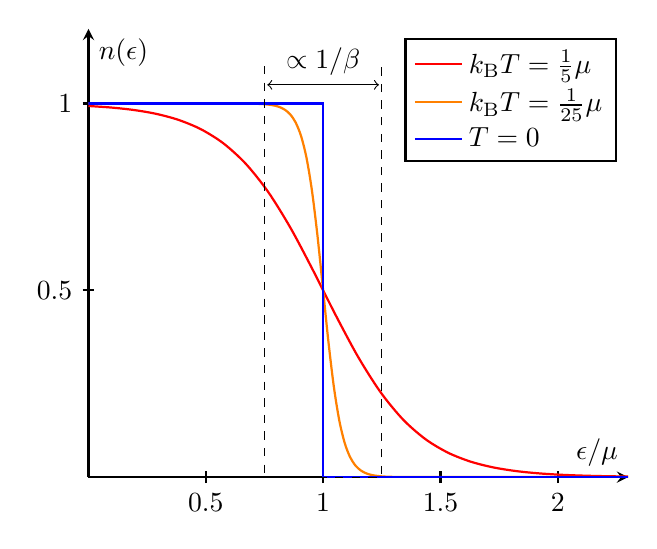
\begin{tikzpicture}
  \begin{axis}[
      xlabel=$\epsilon/\mu$,
      ylabel=$n(\epsilon)$,
      domain=0:\xmax,ymax=\ymax,
      ytick={0.5,1},
      smooth,thick,
      axis lines=center,
      every tick/.style={thick},
      legend cell align=left]

    % Graphs
    \def\chempot{1}
    \def\n#1{1/(e^(#1*(x - \chempot)) + 1)}
    \addplot[color=red]{\n{5}};
    \addplot[color=orange,samples=100]{\n{25}};
    \addplot[const plot,color=blue] coordinates {(0,1) (\chempot,0) (\xmax,0)};

    \legend{$k_\text{B} T = \frac{1}{5} \mu$,$k_\text{B} T = \frac{1}{25} \mu$,$T = 0$}

    % Thermal fluctuations
    \draw [thin,dashed] (\chempot-0.25,1.1) -- (\chempot-0.25,0) -| (\chempot+0.25,1.1);
    \draw [thin,<->,shorten >=1,shorten <=1] (\chempot-0.25,1.05) -- (\chempot+0.25,1.05) node[midway,above] {$\propto 1/\beta$};

  \end{axis}
\end{tikzpicture}
\end{center}

\newpage

\tableofcontents

\newpage

\section{Kinetic Theory of Gases}

This section deals with the \textbf{kinetic theory of gases}, in which we study
the behavior of individual gas atoms and determine quantities such as the
pressure of a gas, the speed probability distribution of atoms, and the rate of
effusion.

\subsection{The Maxwell-Boltzmann Distribution}

Neglecting any rotational or vibrational motion of molecules -- strictly
monotomic gases), the energy of a molecule is given by 

\[
\frac{1}{2}mv_x^2 + \frac{1}{2}mv_y^2 + \frac{1}{2}mv_z^2 = \frac{1}{2}mv^2
\] \vspace{5px}

where $\vec{v} = \langle v_x, v_y, v_z \rangle$ is the molecular velocity and
$v = |\vec{v}|$ is the molecular speed. Our goal is to determine the
distribution of molecular speeds. We will make a couple of assumptions: 

\begin{itemize}
  \item[1.] molecular size $\ll$ intermolecular separation
  \item[2.] ignore any intermolecular forces 
\end{itemize}

\paragraph{The Velocity Distribution} \mbox{} \\

We define the \textbf{velocity distribution function} as the fraction of
molecules with velocities say, in the $x$ direction, between $v_x$ and $v_x
+ dv_x$ as $g(v_x)dv_x$. The velocity distribution function is proportional to
the Boltzmann Factor: 

\[
  p_i \propto e^{\left( -\frac{\varepsilon_i}{kT} \right)}  
\] \vspace{5px}

where $p_i$ is the probability of the system being in state $i$ and
$\varepsilon_i$ is the energy of that state. Therefore, for molecules having
velocities in the $x$ direction, 

\[
  g(v_x) \propto e^{\left( \frac{-mv_x^2}{2kT} \right)} 
\] \vspace{5px}

\begin{center}
\begin{tikzpicture}[scale = 0.75]
  \begin{axis}[
  ylabel =  $g(v_x)$, 
  xlabel =  $v_x$,
  yticklabel=\empty,
  xticklabel=\empty,
  axis lines=left,
  xtick =\empty,
  ytick =\empty
]
\addplot[color=red, samples = 100]{exp(-x^2)};
\end{axis}i
\end{tikzpicture}
\end{center}

The velocity distribution function is sketched above. To normalize this
function ($\int_{-\infty}^{\infty} g(v_x) \, dv_x = 1$), we need to
evaluate this integral: 

\[
  \int_{-\infty}^{\infty} e^{-mv_x^2 / 2kT} \, dv_x = \sqrt{\frac{\pi}{m/2kT}}
  = \frac{2\pi kT}{m}
\] \vspace{5px}

Therefore, 

\[
  g(v_x) = \sqrt{\frac{m}{2\pi kT}} e^{\frac{-mv_x^2}{2kT}}
\] \vspace{5px}

We can then find the following expectation values of this distribution: 

\begin{align*}
  \langle v_x \rangle &= \int_{-\infty}^{\infty} v_x g(v_x) \, dv_x = 0, \\
  \langle |v_x| \rangle &= 2\int_0^\infty v_x g(v_x) \, dv_x
  = \sqrt{\frac{2kT}{\pi m}} \\
  \langle v_x^2 \rangle &= \int_{-\infty}^{\infty} v_x^2 g(v_x) \, dv_x
  = \frac{kT}{m}
\end{align*}
\vspace{5px} 

It does not matter which component of velocity was initially chosen. Hence the
fraction of molecules with velocities between $(v_x, v_y, v_z)$ and $(v_x
+ dv_x, v_y + dv_y, v_z + dv_z)$ is given by

\begin{align*}
  g(v_x)dv_x \, g&(v_y)dv_y \, g(v_z)dv_z \\ 
                 &\propto e^{-mv_x^2 / 2kT} dv_x \, e^{-mv_y^2 / 2kT} dv_y \,
                 e^{-mv_z^2 / 2kT} dv_z \\
                 &= e^{-mv^2 / 2kT} dv_x dv_y dv_z. 
\end{align*}
\vspace{5px}

\paragraph{The Speed Distribution}

To work out the distribution of molecular speeds in a gas, we want the fraction
of molecules which are traveling with speeds between $v = |\vec{v}|$ and $v
+ dv$. This corresponds to a spherical shell in velocity space of radius $v$
and thickness $dv$. 

\begin{figure}[H]
  \centering
    \includegraphics[width = 4.5cm]{screenshot 25.png}
\end{figure}

The volume of velocity space corresponding to speeds between $v$ and $v+dv$ is
therefore equal to 

\[4\pi v^2 \, dv\] 

The fraction of molecules with speeds between $v$ and $v+dv$ is defined as
$f(v)\,dv$, where $f(v)$ is given by 

\[
  \boxed{f(v) \, dv \propto v^2 \, dv \, e^{-mv^2 / 2kT} }
\] \vspace{5px}

To normalize this function ($\int_0^\infty f(v)dv = 1$ ), we evaluate the
integral. Note* the integration bounds are $0\to\infty$ because the speed $v
= |\vec{v}|$ is a positive quantity. 

\[
  \int_0^\infty v^2 e^{-mv^2 / 2kT}\, dv
  = \frac{1}{4}\sqrt{\frac{\pi}{(m/2kT)^3}}
\] \vspace{5px}

Therefore, 

\[
  \boxed{f(v) \, dv = \frac{4}{\sqrt{\pi}} \left( \frac{m}{2kT} \right)^{3/2}
  v^2 \, dv \, e^{-mv^2 / 2kT} }
\] \vspace{5px}

This speed distribution function is known as the  \textbf{Maxwell-Boltzmann
Distribution}. We can now derive some of its properties. 

\paragraph{ $\langle v \rangle$ and $\langle v^2 \rangle$ } \mbox{} \\
\begin{align*}
  \langle v \rangle &= \int_{0}^{\infty} vf(v) \, dv = \sqrt{\frac{8kT}{m}}\\
  \langle v^2 \rangle &= \int_{0}^{\infty} v^2 f(v) \, dv = \frac{3kT}{m}
\end{align*}

This makes sense since, 

\[
\langle v_x^2 \rangle + \langle v_y^2 \rangle + \langle v_z^2 \rangle
= \frac{kT}{m} + \frac{kT}{m} + \frac{kT}{m} = \frac{3kT}{m} = \langle v^2
\rangle
\] \vspace{5px}

The root mean squared speed of a molecule, $v_\text{rms}$ 

\[
  v_\text{rms} = \sqrt{\langle v^2 \rangle} = \sqrt{\frac{3kT}{m}}
\] \vspace{5px}
\paragraph{The Mean Kinetic Energy of a Gas Molecule} \mbox{} \\

The mean kinetic energy of a gas molecule is given by 

\[
  \langle E_{KE} \rangle = \frac{1}{2}m\langle v^2 \rangle = \frac{3}{2}kT
\] \vspace{5px}

This shows that the speed of molecules is proportional to the temperature. The
average energy of a molecule in gas depends \textit{only} on temperature. 

\paragraph{The Maximum of $f(v)$ } \mbox{}\\

The maximum value of $f(v)$ is found by setting 

\[
\frac{d f}{d v} = 0
\] \vspace{5px}

As $f(v)$ 
\[
f(v) = \frac{4}{\sqrt{\pi}} \left( \frac{m}{2kT} \right)^{3/2} v^2 e^{-mv^2
/ 2kT},
\] \vspace{5px}

Differentiating, 

\begin{align*}
  \frac{d f}{d v} &= \frac{4}{\sqrt{\pi}}\left( \frac{m}{2kT} \right)^{3/2}
  \frac{d}{dv} v^2 e^{-mv^2 / 2kT} \\
                  &= \frac{4}{\sqrt{\pi}}\left( \frac{m}{2kT} \right)^{3/2}
                  e^{-mv^2/2kT}\left( -\frac{mv^3}{kT} +2v \right)  
\end{align*}

For $ \frac{df}{dv} = 0$, 

\[
  -\frac{mv^3}{kT} + 2v = 0 \quad \Rightarrow \quad v_\text{max} = \sqrt{\frac{2kT}{m}}
\] \vspace{5px}

And since, 

\[
\sqrt{2} < \sqrt{\frac{8}{\pi}} < \sqrt{3}, 
\] \vspace{5px}

we have that 

\[
  v_\text{max} < \langle v \rangle < v_\text{rms}
\] \vspace{5px}

Note* $v_\text{max}$ is not the maximum velocity a particle can have -- it is the
\textit{most probable} velocity a particle would have. 


\begin{figure}[H]
  \centering
    \includegraphics[width = 6cm]{screenshot 26.png}
\end{figure}

\subsection{Chapter Summary}

A physical situation that is very important in kinetic theory is the
\textit{translational} motion of atoms or molecules in a gas. The probability
distribution for a given component of velocity is given by 

\[
  g(v_x) \propto e^{-mv_x^2 / 2kT}
\] \vspace{5px}

The corresponding expression for the probability distribution for molecular
speeds is given by 

\[
  f(v) \propto v^2e^{-mv^2 / 2kT}
\] \vspace{5px}

This is known as the \textbf{Maxwell-Boltzmann Distribution}. Two important
average values of the Maxwellian Distribution are: 
 \[
\langle v \rangle = \sqrt{\frac{8kT}{\pi m}}, \qquad \langle v^2 \rangle
= \frac{3kT}{m}
\] \vspace{5px}

The maximum likelihood velocity a gas molecule has: 

\[
  v_\text{max} = \sqrt{\frac{2kT}{m}}
\] \vspace{5px}

The rms velocity of a gas molecule, $v_\text{rms} = \sqrt{\langle v^2 \rangle}$ 

\[
  v_\text{rms} = \sqrt{\frac{3kT}{m}}
\] \vspace{5px}











\end{document}

